\documentclass[a4j,twoside,openright,11pt]{jarticle}
%
\usepackage{amsmath,amssymb}
\usepackage{bm}
\usepackage{graphicx}
\usepackage{ascmac}
\usepackage{listliketab}
\usepackage{url}
\usepackage{listings}

\setlength{\textwidth}{15.92cm}
\setlength{\oddsidemargin}{0mm}
\setlength{\evensidemargin}{0mm}
\setlength{\topmargin}{-1cm}
\setlength{\textheight}{23.5cm}
\setlength{\footskip}{18mm}

%
\pagestyle{plain}
\makeatletter
  \def\@maketitle{%
  \newpage\null
  \vskip 2em%
  \begin{center}%
  \let\footnote\thanks
    {\Large \@title \par}%
    \vskip 1.5em%
  \end{center}% 追加
  \begin{flushright}
        \@author
  \end{flushright}
  \begin{flushright}% 追加
    {\large \@date}%
  \end{flushright}%
  \par\vskip 1.5em}
\makeatother

\title{伝熱実験\\--熱電対を使った温度計測と熱伝導実験及び熱交換器実験--\\2.熱交換実験}
\author{九州工業大学 機械知能工学科 機械コース\\3年 学籍番号:13104069 坂本 悠作}
\date{
実験日2:平成27年7月\,\,\,\,8日\\
提出日 :平成27年7月15日\\
共同実験者\\
川内 諒\\
川上 晃弘\\
金城 悟\\
草場 悠真\\
石井 敦\\
一ノ宮 浩祐\\
砂野 仁輝\\
高野 真里\\
是永 遼介\\
酒井 淳\\
里中 花実\\
白石 大輔\\
高木 怜\\
}
\begin{document}
\maketitle
\newpage

\section{目的}
並流型及び交流型熱交換器について、対数平均温度差、熱通過率、及び温度効率を実験により求め、熱伝達理論と実験の比較、実験結果の整理方法を学ぶ.
\section{レポート課題}
\subsection{次元解析から$Nu=CRe^mPr^n$を導く(バッキンガムの$\pi$定理を利用)。また、ヌセルト数、レイノルズ数、プラントル数の物理的意味を調べる。}
\subsubsection{バッキンガムの$\pi$定理}
バッキンガムの$\pi$定理は、n個の物理量とm個の基本物理量が存在するとき、(n-m)個の無次元量で表現できるという定理。熱伝導実験で関係がある物理量を表1に示す。
\begin{table}[htb]
\begin{center}
  \caption{物理量}
  \begin{tabular}{lcc} \hline
物理量&記号&MLST次元式\\\hline
熱伝達率&h&$M/(S^3T)$\\
流体の密度&$\rho$&$M/L^3$\\
定圧比熱&$C_p$&$L^2/(S^2)$\\
代表寸法&l&L\\
流体の熱伝導率&$\lambda$&$ML/(S^3T)$\\
流速&w&L/S\\
流体の粘性係数&$\mu$&$M/(LS)$\\
\hline
  \end{tabular}
\end{center}
\end{table}
\begin{eqnarray}
Nu = \frac{hd}{\lambda} =0.023Re^{0.8}Pr^{\frac{1}{3}}
\end{eqnarray}

これら7つの物理量に対して、次の式が成立する
\begin{eqnarray}
f(h,\rho,C_p,l,\lambda,w,\mu) = 0
\end{eqnarray}
よって、(物理量-基本物理量)=(7-4)=3となるので、3つの無次元数を用いて
\begin{eqnarray}
f(\pi_1,\pi_2,\pi_3) = 0
\end{eqnarray}
\subsubsection{ヌセルト数の導出}
ヌセルト数は、熱伝達率hに関する無次元量であるので、$l,\lambda,w,\mu$を用いて無次元化していく。無次元量$\pi_1$とhの間には、次の関係があるとする。
\begin{eqnarray}
\pi_1 = \frac{h}{l^a \lambda^b w^c \mu^d}
\end{eqnarray}
MLST次元量で書き直すと、
\begin{eqnarray}
\pi_1[\cdot] = \frac{M^1S^{-3}T^{-1}}{M^{b+d} L^{a+b+c-d} S^{-3b-c-d} T^{-b}}
\end{eqnarray}
よって、連立方程式が成り立つ。
\begin{eqnarray}
b+d = 1\nonumber\\
a+b+c-d = 0\nonumber\\
-3b-c-d = -3\nonumber\\
-b = -1\nonumber
\end{eqnarray}
これを解いて、a=-1,b=1,c=0,d=0となる。よって、
\begin{eqnarray}
\pi_1 = \frac{hl}{\lambda}= Nu
\end{eqnarray}
同様に、
\begin{eqnarray}
\pi_2 = \frac{wl\rho}{\mu}= Re\\
\pi_3 = \frac{C_p\mu}{\lambda}= Pr
\end{eqnarray}

以上より、
\begin{eqnarray}
\pi_1 &=& f(\pi_2,\pi_3)\nonumber\\
Nu    &=& f(Re,Pr)\nonumber\\
      &=& CRe^mPr^n (C,m,nは定数)
\end{eqnarray}

\subsubsection{物理的意味}
\begin{enumerate}
\item ヌセルト数\\
対流熱伝導の際に、壁面での温度勾配を基準温度勾配で除したもの。このあたいが大きければ壁面でより急峻な変化をしており、逆に小さければ壁面での変化は緩やかになる。
\begin{eqnarray}
Nu = \frac{hd}{\lambda}
\end{eqnarray}
\item レイノルズ数\\
流れの特性を表す無次元数で、層流か乱流かを判断する量。分子は慣性力、分母は粘性を示す量で、乱流が発生しにくい環境(慣性力が小さく、粘性が大きい)ではレイノルズ数は小さくなる。
\begin{eqnarray}
Re = \frac{\rho u l}{\mu}
\end{eqnarray}
\item プラントル数\\
流れと熱移動の相関を表す無次元数。温度境界層と速度境界層の関係を注目した場合、速度境界層に対して温度境界層の方が大きければ、Pr$<$1となり、速度境界層に温度境界層が一致していればPr=1,温度境界層の方が小さければPr$>$1となる。
\begin{eqnarray}
Pr = \frac{\nu}{\alpha} =\frac{c_p\mu}{\lambda}
\end{eqnarray}
\end{enumerate}

\subsection{両対数グラフの縦軸に$Nu/Pr^n$,横軸にReを取り、実験データをプロットし、最小二乗法から係数決定をし、実験式を求める。}
Colburnの実験式($L/D>60$の範囲で適用できる理論式)
\begin{eqnarray}
Nu = \frac{hd}{\lambda} =0.023Re^{0.8}Pr^{\frac{1}{3}}
\end{eqnarray}

理論式より、
\begin{eqnarray}
Nu/Pr^{1/3}=CRe^m (C,mは定数)\nonumber
\end{eqnarray}
であるので、誤差の自乗が最小となるようなC,mを求める。$y=\log (Nu/Pr^{1/3}),x=Re,\alpha = m,\beta = \log(C)$とすれば、伝熱実験で使用したプログラムを用いて求めることができる。
\begin{eqnarray}
  Nu/Pr^{1/3}=10^{-1.77002}Re^{0.810572}
\end{eqnarray}

\begin{figure}[htbp]
\begin{center}
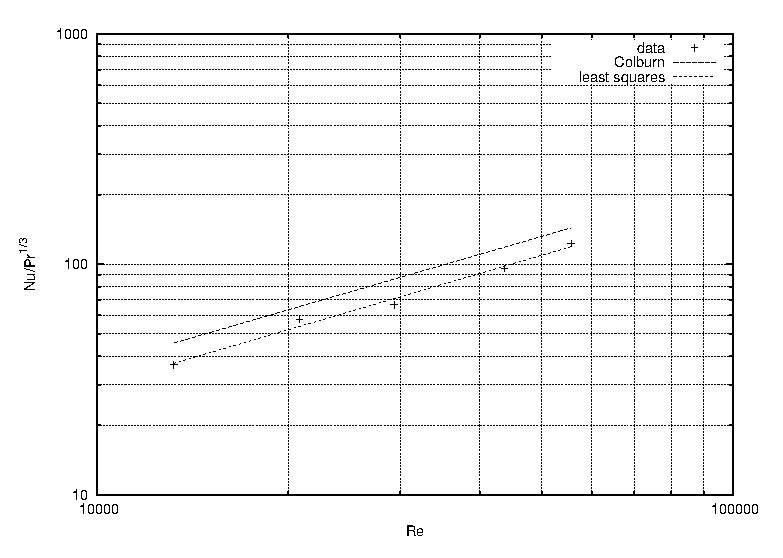
\includegraphics[width=14cm]{./Colburn/data.eps}
\end{center}
\caption{レポート課題2}
\end{figure}

\subsection{課題2で求めた実験データとコルバーンの式を比較し考察する。}
\begin{table}[htb]
\begin{center}
  \caption{比較表}
  \begin{tabular}{|l|c|c|} \hline
$Nu/Pr^{1/3}$実験式&$Nu/Pr^{1/3}$Colburnの式&誤差(Colburn基準[\%])\\
\hline
123.0&143.942&85.45\\
96.01&118.675&80.90\\
66.6 & 86.221&77.24\\
57.73& 65.528&88.10\\
36.56& 45.557&80.25\\\hline
  \end{tabular}
\end{center}
\end{table}
全体的にコルバーンの式よりも小さい値となった。誤差の大きいもので最大23\%、小さいもので12\%という結果になった。

コルバーンの式は、乱流で壁温が一定、プラントル数が一定、円管流れの条件での関係を表している関係式である。この実験式とコルバーンの式はよく似たものであるので、実際の関係式をよく表現できている式であると考えられる。

\subsection{並流型、向流型熱交換器の性能について調べ、まとめる}
\subsubsection{並流型熱交換器}
高温流体と低温流体が同じ方向に流動する熱交換器である。両流体入り口近傍で大きな温度差が生じるので、素早い熱交換が行えるが、低温流体の出口温度が高温流体の出口温度を超えることはない。

\subsubsection{向流型熱交換器}
高温流体と低温流体が互いに反対方向に流動する熱交換器であり、両流体間の温度差が小さくなるため、大量の熱交換をさせるためには大きな熱通過面積が必要になるが、低温流体を高温流体の出口以上に加熱することが可能である。\\
\par

\subsubsection{冷却水4大障害}
冷却水では腐食によるチューブの損傷、熱交換率の低下などを引き起こす問題が生じるため、冷却水の適切な水質管理が重要になる。
\begin{enumerate}
\item 腐食障害\\
腐食と水質には密接な関係があり、腐食が進むと穴あき等がおこる。
\item スライム障害\\
微生物が繁殖し、その微生物が分泌する粘性有機物がスライムの原因である。
\item スケール障害\\
不溶解成分で、局部腐食を引き起こすほか、熱交換率を低下させる。
\item レジオネラ障害\\
レジオネラ菌を空気中に放出するため、感染症に注意する必要がある。
\end{enumerate}

\section{まとめ}
この実験では、熱交換器の挙動についてデータを取り、Colburnの式と比較した。ヌセルト数、レイノルズ数、プラントル数の定義と物理的意味について学んだ。

\section{参考文献}
\begin{enumerate}
\item \url{http://www.sit.ac.jp/user/konishi/JPN/L_Support/SupportPDF/Non-dimension.pdf}
\item \url{http://envuniv.net/bakkingam.php}
\item \url{http://web2.clarkson.edu/projects/subramanian/ch330/notes/Heat%20Transfer%20in%20Flow%20Through%20Conduits.pdf}
\item \url{https://www.google.co.jp/url?sa=t&rct=j&q=&esrc=s&source=web&cd=5&ved=0CDQQFjAEahUKEwiSipT43Y7HAhUJkpQKHdSYBqo&url=http%3A%2F%2Fwww.ocw.titech.ac.jp%2Findex.php%3Fmodule%3DGeneral%26action%3DDownLoad%26file%3D2004-6550-20041116-3-8.pdf%26type%3Dcal%26JWC%3D200826550&ei=xVLAVdKTOomk0gTUsZrQCg&usg=AFQjCNGkS0r48c3y1oFkcE_SDKf8G-jp_g}
\item \url{http://www.mizu-shori.com/solution/}
\end{enumerate}

\end{document}
